\documentclass{article}
\usepackage{tikz}
\usepackage{svg}
\usepackage{graphicx}
\usepackage[landscape,paper=a4paper,margin=10pt]{geometry}

\usetikzlibrary{decorations.pathreplacing}

\newcommand{\doubleunderline}[1]{%
  \tikz[baseline=(X.base)]{
    \node[inner sep=0pt, outer sep=0pt] (X) {\strut #1};
    \draw[line width=0.3pt, dash pattern=on 2pt off 1pt] ([yshift=-2pt]X.south west) -- ([yshift=-2pt]X.south east);
    \draw[line width=0.3pt, solid] ([yshift=-4pt]X.south west) -- ([yshift=-4pt]X.south east);
  }%
}
\newcommand{\solidunderline}[1]{%
  \tikz[baseline=(X.base)]{
    \node[inner sep=0pt, outer sep=0pt] (X) {\strut #1};
    \draw[line width=0.3pt, solid] ([yshift=-2pt]X.south west) -- ([yshift=-2pt]X.south east);
  }%
}
\newcommand{\dashedunderline}[1]{%
  \tikz[baseline=(X.base)]{
    \node[inner sep=0pt, outer sep=0pt] (X) {\strut #1};
    \draw[line width=0.3pt, dash pattern=on 2pt off 1pt] ([yshift=-1pt]X.south west) -- ([yshift=-1pt]X.south east);
  }%
}
\pagestyle{empty}
\begin{document}
\begin{center}
  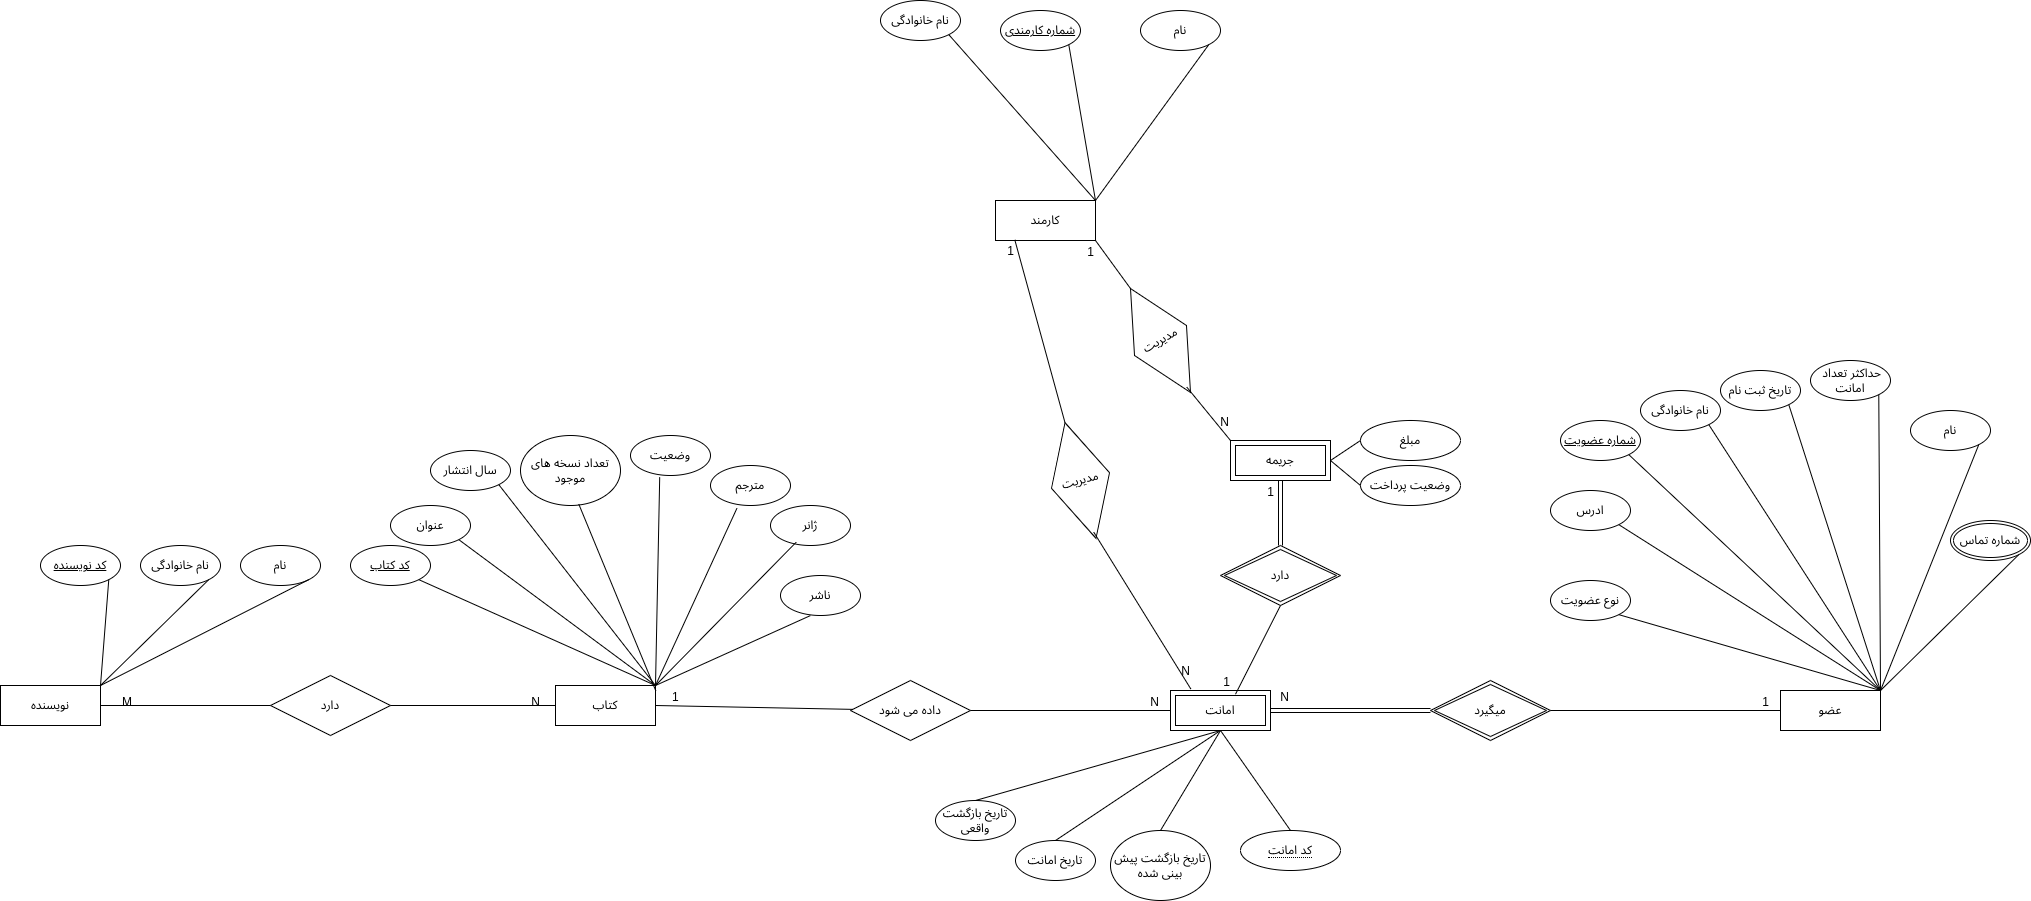
\includegraphics[height=\dimexpr\paperheight-20pt\relax,width=\dimexpr\paperwidth-20pt\relax,keepaspectratio=true]{./faze1/database.png}
\end{center}
\newpage
\noindent
\textbf{Database Design :}
\newline\newline
Writer(\solidunderline{WriterID}, Name,LastName)
\newline\newline
Book(\solidunderline{BookID}, Title,Publisher, PublishedYear, NumberOfCopies, Translator, Genre, State)
\newline\newline
WriterBook(\solidunderline{\dashedunderline{WriterID}, \dashedunderline{BookID}})
\newline\newline
Member(\solidunderline{MemberID}, Name, LastName, Address, RegistrationDate, MaximumNumberOfBorrowedBooks, TypeOfMembership)
\newline\newline
PhoneNumbers(\solidunderline{\dashedunderline{MemberID}, PhoneNumber})
\newline\newline
Employee(\solidunderline{EmployeeID}, Name, LastName)
\newline\newline
BookBorrowed(\solidunderline{\dashedunderline{MemberID}, \dashedunderline{BookID}, BookBorrowedID}, BorrowedDate, ReturnDate, PredictedReturnDate, \dashedunderline{ManagedByEmployeeID})
\newline\newline
LateReturnFine(\doubleunderline{\dashedunderline{MemberID}, \dashedunderline{BookID}, BookBorrowedID}, FineAmount, PaymentStatus ,\dashedunderline{ManagedByEmployeeID})
\end{document}